%%%%%%%%%%%%%%%%%%%%%%%%%%% asme2e.tex %%%%%%%%%%%%%%%%%%%%%%%%%%%%%%%%%
% Template for producing ASME-format articles using LaTeX            %
% Written by   Harry H. Cheng                                        %
%              Integration Engineering Laboratory                    %
%              Department of Mechanical and Aeronautical Engineering %
%              University of California                              %
%              Davis, CA 95616                                       %
%              Tel: (916) 752-5020 (office)                          %
%                   (916) 752-1028 (lab)                             %
%              Fax: (916) 752-4158                                   %
%              Email: hhcheng@ucdavis.edu                            %
%              WWW:   http://iel.ucdavis.edu/people/cheng.html       %
%              May 7, 1994                                           %
% Last change: December 5, 1998                                      %
% Use at your own risk, send complaints to /dev/null                 %
%%%%%%%%%%%%%%%%%%%%%%%%%%%%%%%%%%%%%%%%%%%%%%%%%%%%%%%%%%%%%%%%%%%%%%

%%% use two columns and ASME format
\documentclass[twocolumn,10pt]{asme2e}

%\linespread{1.8}  %%%Double space lines (remove for final draft)
\usepackage{graphicx}
\usepackage{ifthen}
\usepackage{dcolumn}% Align table columns on decimal point
\usepackage{multirow}
\usepackage{booktabs}
\usepackage{bm}% bold math
\usepackage{amsbsy}
\usepackage{amsmath}


\newcommand{\SUM}[2]{\ifthenelse{\equal{#1}{0}}{\sum_{\alpha_{#2},b_{#2},l_{#2}}^{3,n,N}} {\ifthenelse{\equal{#1}{1}}{\sum_{\alpha_{#2},b_{#2}}^{3,n}}{\sum_{\pmb{\kappa}#2,\nu#2}^{N,3n}}}}

\newcommand{\EXP}[1]{\exp\mspace{-5.0mu}\left[#1\right]\mspace{-3.0mu}}

\newcommand{\abcdt}[5]{\mspace{-4.0mu}\left(\mspace{-8.0mu}\begin{smallmatrix}&\ifthenelse{\equal{#1}{}}{a}{#1}&\ifthenelse{\equal{#3}{}}{c}{#3}\\&\ifthenelse{\equal{#2}{}}{b}{#2}&\ifthenelse{\equal{#4}{}}{d}{#4}\end{smallmatrix}\mspace{-2.0mu};\ifthenelse{\equal{#5}{}}{t}{#5}\right)}

\newcommand{\abcd}[4]{\mspace{-4.0mu}\left(\mspace{-8.0mu}\begin{smallmatrix}&\ifthenelse{\equal{#1}{}}{a}{#1}&\ifthenelse{\equal{#3}{}}{c}{#3}\\&\ifthenelse{\equal{#2}{}}{b}{#2}&\ifthenelse{\equal{#4}{}}{d}{#4}\end{smallmatrix}\mspace{-3.0mu}\right)}

\newcommand{\abt}[3]{\mspace{-4.0mu}\left(\mspace{-8.0mu}\begin{smallmatrix}&\ifthenelse{\equal{#1}{}}{a}{#1} \\&\ifthenelse{\equal{#2}{}}{b}{#2}\end{smallmatrix}\mspace{-2.0mu};\ifthenelse{\equal{#3}{}}{t}{#3}\right)}

\newcommand{\ab}[2]{\mspace{-4.0mu}\left(\mspace{-8.0mu}\begin{smallmatrix}&\ifthenelse{\equal{#1}{}}{a}{#1} \\&\ifthenelse{\equal{#2}{}}{b}{#2}\end{smallmatrix}\mspace{-3.0mu}\right)}

\newcommand{\kvbat}{\mspace{-4.0mu}\left(\mspace{-8.0mu}\begin{smallmatrix} &\pmb{\kappa} &b \\ &\nu &\alpha\end{smallmatrix}\mspace{-2.0mu};t\right)}

\newcommand{\kvbaw}{\mspace{-4.0mu}\left(\mspace{-8.0mu}\begin{smallmatrix} &\pmb{\kappa} &b \\ &\nu &\alpha\end{smallmatrix}\mspace{-2.0mu};\omega\right)}

\newcommand{\kvba}{\mspace{-4.0mu}\left(\mspace{-8.0mu}\begin{smallmatrix} &\pmb{\kappa} &b \\ &\nu &\alpha\end{smallmatrix}\mspace{-3.0mu}\right)}

\newcommand{\kvt}{\mspace{-4.0mu}\left(\mspace{-8.0mu}\begin{smallmatrix}&\pmb{\kappa} \\&\nu\end{smallmatrix}\mspace{-2.0mu};t\right)}

\newcommand{\kvw}{\mspace{-4.0mu}\left(\mspace{-8.0mu}\begin{smallmatrix}&\pmb{\kappa} \\&\nu\end{smallmatrix}\mspace{-2.0mu};\omega\right)}

\newcommand{\kv}{\mspace{-4.0mu}\left(\mspace{-8.0mu}\begin{smallmatrix}&\pmb{\kappa} \\&\nu\end{smallmatrix}\mspace{-3.0mu}\right)}

\newcommand{\lbt}{\mspace{-4.0mu}\left(\mspace{-8.0mu}\begin{smallmatrix}&l \\&b\end{smallmatrix}\mspace{-2.0mu};t\right)}

\newcommand{\lb}{\mspace{-4.0mu}\left(\mspace{-8.0mu}\begin{smallmatrix}&l \\&b\end{smallmatrix}\mspace{-3.0mu}\right)}



%%% Replace here with information related to your conference
\confshortname{AJTEC2011}
%\conffullname{the 8$^{\rm th}$ ASME-JSME Thermal Engineering Joint Conference}
\conffullname{the ASME/JSME 2011 8$^{\rm th}$ Thermal Engineering Joint Conference}

%%%%% for date in a single month, use
\confdate{13-17}
\confmonth{March}
%%%%% for date across two months, use
%\confdate{August 30-September 2}
\confyear{2011}
\confcity{Honolulu, Hawaii}
\confcountry{USA}

%%% Replace DETC2010/MECH-12345 with the number supplied to you
%%% by ASME for your paper.
\papernum{AJTEC2011-44315}

\title{PREDICTING PHONON PROPERTIES FROM MOLECULAR DYNAMICS SIMULATIONS USING THE SPECTRAL ENERGY DENSITY}

%%% first author
\author{Joseph E. Turney\\
\textbf{John A. Thomas}\\
\textbf{Alan J. H. McGaughey}\thanks{Address all correspondence to this author.}
    \affiliation{
    Department of Mechanical Engineering\\
    Carnegie Mellon University\\
    Pittsburgh, Pennsylvania 15213-3890\\
    Email: mcgaughey@cmu.edu
    }
}

%%% second author (this is what is printed)
%%% remove the following entry for single author
%%% add more entries for multiple authors
\author{Cristina H. Amon
	\affiliation{
    Department of Mechanical Engineering\\
    Carnegie Mellon University\\
    Pittsburgh, Pennsylvania 15213-3890\\
    }
    \affiliation{
	Department of Mechanical \& Industrial Engineering\\
    University of Toronto\\
    Toronto, Ontario M5S 3G8
    }
}

\begin{document}

\maketitle

%%%%%%%%%%%%%%%%%%%%%%%%%%%%%%%%%%%%%%%%%%%%%%%%%%%%%%%%%
\begin{abstract}
\textit{Using lattice dynamics theory, we derive the spectral energy density
and the relation between the spectral energy density and the phonon
frequencies and relaxation times.  We then calculate the spectral energy
density and phonon frequencies and relaxation times for a test system of
Lennard-Jones argon using velocities obtained from molecular dynamics
simulations. The phonon properties, which can be used to calculate thermal
conductivity, are compared to predictions made using (i) anharmonic lattice
dynamics calculations and (ii) a technique that performs normal mode analysis
on the positions and velocities obtained from molecular dynamics
simulations.}
\end{abstract}

%%%%%%%%%%%%%%%%%%%%%%%%%%%%%%%%%%%%%%%%%%%%%%%%%%%%%%%%%
%\begin{nomenclature}

%\entry{$a$}{lattice parameter}


%\subsection*{Greek}

%\entry{$\alpha$}{thermal expansion coefficient}


%\subsection*{Subscripts}

%\entry{$i$, $j$, $k$}{atomic indices}


%\end{nomenclature}


%%%%%%%%%%%%%%%%%%%%%%%%%%%%%%%%%%%%%%%%%%%%%%%%%%%%%%%%%
\section*{INTRODUCTION}

Due to the increasing prevalence of nanostructured electronic and
optoelectronic devices and the desire to employ nanostructuring to tune
material properties, it is vital to develop an understanding of the physics
of carrier transport. Phonons are the dominant energy carriers in insulators
and semiconductors, which are integral to many nanostructured devices. While
substantial effort has gone into developing adequate theories of phonon
transport, the current understanding is lacking, even in bulk materials. For
example, which phonon modes dominate energy transport and the importance of
interactions involving four or more phonons are typically unknown.  The
situation only becomes more complicated in nanostructures, where the energy
carriers also interact with surfaces and interfaces.

The usefulness of analytical models of thermal transport has been hampered by
the necessary approximations and assumptions (e.g., a Debye solid, ignoring
optical phonons), permitting only qualitative or semi-quantitative
predictions \cite{callaway1959,holland1963}. When used with the Green-Kubo or
direct methods, molecular dynamics (MD) simulations can predict thermal
conductivity \cite{mcgaughey2004c,landry2008,schelling2002,sellan2010a}.
Because the analysis in these two methods is performed at the system level,
however, no information about the phonons is obtained. The phonon properties
needed to calculate thermal conductivity (group velocities, relaxation times)
can be predicted using MD simulation and normal mode analysis
\cite{ladd1986,mcgaughey2004c,henry2008,goicochea2010}, but this method
requires {\em a priori} knowledge of the phonon frequencies and polarization
vectors and is time-intensive. Phonon frequencies and relaxation times can be
obtained from harmonic and anharmonic lattice dynamics (LD)
calculations,\cite{maradudin1962,wallace1972,ladd1986,dove1993,turney2009a}
but these are theoretically and computationally complex and only valid at low
temperatures.

The spectral energy density
(SED)\cite{marayuma2003,shiomi2006,dekoker2009,thomas2010c}, which we discuss
herein, presents a straightforward alternative by which phonon frequencies
and relaxation times can be obtained using only atomic velocities from an MD
simulation as input. In what follows, we derive the SED from lattice dynamics
theory. We also derive the relation between the SED and the phonon
frequencies and relaxation times. We then calculate the SED using results
from MD simulations of a test system of Lennard-Jones argon and compare the
predicted phonon properties to predictions made using (i) anharmonic LD
calculations and (ii) normal mode analysis performed on the results of the MD
simulations.

\section*{THE SPECTRAL ENERGY DENSITY}\label{S:SED}

\subsection*{Derivation}\label{SS:derivation}

To derive the SED, we begin with results from standard harmonic LD theory.
The system Hamiltonian is\cite{turneythesis},
\begin{equation}\label{E:H_HLD}
\begin{split}
H=&\frac{1}{2}\SUM{}{}\left[\dot{q}^*\kvt \dot{q}\kvt + \omega_0^2\kv q^*\kvt q\kvt\right]\\
 =&\SUM{}{}\left[T\kvt + V\kvt\right],
 \end{split}
\end{equation}
where $t$ is time, $\omega_0\kv$ is the frequency of the phonon denoted by
wave vector $\pmb{\kappa}$ and dispersion branch $\nu$, and $N$ and $n$ are
the total number of unit cells and number of atoms in the unit cell.  The
Hamiltonian is the total system energy and is the sum of the mode- and
time-dependent kinetic and potential energies, $T\kvt$ and $V\kvt$.  The
phonon mode (normal mode) coordinate and its time derivative are given by
\begin{equation}\label{E:q_HLD}
q\kvt=\SUM{0}{}\sqrt{\frac{m_b}{N}}u_{\alpha}\lbt e^*\kvba\EXP{i\pmb{\kappa}\cdot\mathbf{r}_0\ab{l}{0}},
\end{equation}
and
\begin{equation}\label{E:qdot_HLD}
\dot{q}\kvt{}{}{}=\SUM{0}{}\sqrt{\frac{m_b}{N}}\dot{u}_{\alpha}\lbt e^*\kvba\EXP{i\pmb{\kappa}\cdot\mathbf{r}_0\ab{l}{0}},
\end{equation}
where $m_b$ is the mass of the $b^{\textrm{th}}$ atom in the unit cell, and
$\mathbf{r}_0\ab{l}{0}$ is the equilibrium position vector of the
$l^{\textrm{th}}$ unit cell. The $\alpha$-component of the displacement (from
equilibrium), $u_{\alpha}\lbt$, and velocity, $\dot{u}_{\alpha}\lbt$, of the
$b^{\textrm{th}}$ atom in the $l^{\textrm{th}}$ unit cell are time-dependent
and are related to the phonon mode coordinates through the time-independent
polarization vector $e\kvba$. The asterisk superscript in Eqs$.$
\eqref{E:q_HLD} and \eqref{E:qdot_HLD} denotes the complex conjugate.

The allowed wave vectors are defined by the crystal lattice, however, the
phonon frequencies and polarization vectors are not known.  It is convenient
to let $\SUM{1}{}q\kvbat=q\kvt$ and recast Eqs$.$ \eqref{E:H_HLD},
\eqref{E:q_HLD}, and \eqref{E:qdot_HLD} as
\begin{equation}\label{E:H_new}
\begin{split}
H=&\frac{1}{2}\SUM{}{}\SUM{1}{}\left[\dot{q}^*\kvbat \dot{q}\kvbat + \omega_0^2\kvba q^*\kvbat q\kvbat\right]\\
 =&\SUM{}{}\SUM{1}{}\left[T\kvbat + V\kvbat\right],
\end{split}
\end{equation}
\begin{equation}\label{E:q_new}
q\kvbat=e\kvba\sqrt{\frac{m_b}{N}}\sum_l^Nu_{\alpha}\lbt \EXP{i\pmb{\kappa}\cdot\mathbf{r}_0\ab{l}{0}},
\end{equation}
and
\begin{equation}\label{E:qdot_new}
\dot{q}\kvbat=e\kvba\sqrt{\frac{m_b}{N}}\sum_l^N\dot{u}_{\alpha}\lbt \EXP{i\pmb{\kappa}\cdot\mathbf{r}_0\ab{l}{0}}.
\end{equation}
The coordinates $q\kvbat$ are associated with atom $b$ and direction
$\alpha$. In arriving at Eq$.$ \eqref{E:H_new}, we make use of the fact that
$e\kvba=e^*\abcd{-\pmb{\kappa}}{\nu}{b}{\alpha}$ and
$q\kvt=q^*\abt{-\pmb{\kappa}}{\nu}{t}$ \cite{dove1993} to pull the summations
over $\alpha$ and $b$ out of the multiplications in Eq$.$ \eqref{E:H_HLD}.

The average kinetic energy of the crystal is
\begin{equation}\label{E:ave_T_t}
\langle T\kvbat\rangle=\frac{1}{2}\lim_{\tau_0\rightarrow\infty}\frac{1}{2\tau_0}\int_{-\tau_0}^{\tau_0}\dot{q}^*\kvbat\dot{q}\kvbat dt.
\end{equation}
The kinetic energy can be transformed from the time domain ($t$) to the
frequency domain ($\omega$) by Parseval's theorem\cite{rudin1987},  allowing
Eq$.$ \eqref{E:ave_T_t} to be written as
\begin{equation}\label{E:ave_T_w1}
\langle T\kvbaw\rangle=\lim_{\tau_0\rightarrow\infty}\frac{1}{4\tau_0}\left|\frac{1}{\sqrt{2\pi}}\int_{-\tau_0}^{\tau_0}\dot{q}\kvbat\exp(-i\omega t)dt\right|^2.
\end{equation}
Substituting the expression for $\dot{q}\kvbat$ [Eq$.$ \eqref{E:qdot_new}] into Eq$.$ \eqref{E:ave_T_w1}, we obtain
\begin{multline}\label{E:ave_T_w}
\langle T\kvbaw\rangle=\frac{m_b|e\kvba|^2}{8\pi\tau_0N}\\
\times\left|\int_{-\tau_0}^{\tau_0}\sum_l^N\dot{u}_{\alpha}\lbt\EXP{i\pmb{\kappa}\cdot\mathbf{r}_0\ab{l}{0}-i\omega t}dt\right|^2,
\end{multline}
where, for brevity, the limit has been dropped.

The spectral energy density (i$.$e$.$, the total system energy in the frequency domain) is
\begin{equation}\label{E:SED}
\begin{split}
\Phi&(\omega,\pmb{\kappa})=2\sum_{\nu}^{3n}\sum_{\alpha,b}^{3,n}\langle T\kvbaw\rangle\\
                         =&\frac{1}{4\pi\tau_0N}\sum_b^nm_b\sum_{\alpha}^3\left|\int_{-\tau_0}^{\tau_0}\sum_l^N\dot{u}_{\alpha}\lbt\EXP{i\pmb{\kappa}\cdot\mathbf{r}_0\ab{l}{0}-i\omega t}dt\right|^2,
\end{split}
\end{equation}
where we have used the fact that the eigenvectors are orthonormal (i$.$e$.$,
$\sum_{\nu}^{3n}|e\kvba|^2=1$)\cite{dove1993} and equipartition of energy
(valid for a classical, harmonic system). Given the atomic velocities in a
system, the spectral energy density can be calculated at arbitrary
frequencies for the allowed wave vectors. The Hamiltonian can be written as
\begin{equation}\label{E:equipartition}
H=\sum_{\pmb{\kappa}}^{N}\int_{-\infty}^{\infty}\Phi(\omega,\pmb{\kappa})d\omega=2\sum_{\pmb{\kappa},\nu}^{N,3n}\sum_{\alpha,b}^{3,n}\langle T\kvbat\rangle.
\end{equation}


\subsection*{Relation to Phonon Properties}\label{S:Properties}

In an anharmonic system, the phonon populations fluctuate about the
equilibrium distribution function. The phonon mode coordinates and their time
derivatives are
\begin{equation}\label{E:q_A}
q_A\kvt=\left[q_{SS}\kvt+q_{T}\kvt\right]
\end{equation}
and
\begin{equation}\label{E:qdot_A}
\dot{q}_A\kvt=\left[\dot{q}_{SS}\kvt+\dot{q}_{T}\kvt\right].
\end{equation}
The steady-state and transient parts and their time derivatives are given by
\begin{equation}\label{E:q_A_SS}
q_{SS}\kvt=C_1\kv\exp\lbrace i\omega_A\kv t\rbrace+C_2\kv\exp\lbrace -i\omega_A\kv t\rbrace,
\end{equation}
\begin{equation}\label{E:q_A_T}
q_{T}\kvt=\EXP{-\Gamma\kv |t|}\lbrace C_3\kv\EXP{i\omega_A\kv t}-C_4\kv\EXP{-i\omega_A\kv t}\rbrace,
\end{equation}
\begin{equation}\label{E:qdot_A_SS}
\dot{q}_{SS}\kvt=i\omega_A\kv\left\{C_1\kv\exp[i\omega_A\kv t]-C_2\kv\exp[-i\omega_A\kv t]\right\},
\end{equation}
and
\begin{multline}\label{E:qdot_A_T}
\dot{q}_{T}\kvt=\EXP{-\Gamma\kv |t|}\left\{C_3\kv\left[i\omega_A\kv-\Gamma\kv\right]\EXP{i\omega_A\kv t}\right.
\\\left.-C_4\kv\left[i\omega_A\kv+\Gamma\kv\right]\EXP{-i\omega_A\kv t } \right\},
\end{multline}
where the $C$s are constants and $\omega_A\kv$ and $\Gamma\kv$ are the phonon
mode frequency and scattering rate (i$.$e$.$, linewidth).  The transient part
describes the creation of an excess in the population of a phonon mode for
$t<0$ and its decay back to equilibrium for $t>0$.

The model used for anharmonic lattice dynamics is an excitation and decay of
a single phonon mode.  In a real system, there will be multiple phonons in
each mode that simultaneously grow or decay with time.  Thus, (dealing only
with $\dot{q}$) we let
\begin{multline}\label{E:qdot_A_kvbat}
\dot{q}\kvt=\sum_j i\EXP{-\Gamma\kv |t-t_j|}\\
\times\lbrace A_j\kv\left[\omega_A\kv+i\Gamma\kv\right]\EXP{i\omega_A\kv (t-t_j)}
\\-B_j\kv \left[\omega_A\kv-i\Gamma\kv\right]\EXP{-i\omega_A\kv (t-t_j)}\rbrace,
\end{multline}
where many phonons in each mode, indexed by $j$, are simultaneously being
created and destroyed.  The phonons grow for $t<t_j$ and decay for $t>t_j$
and $A_j$ and $B_j$ are constants.  We are  not concerned with the values of
$t_j$, $A_j$, and $B_j$, though they should take on values such that
$\langle\dot{q}_{SS}^*\kvt\dot{q}_{SS}\kvt\rangle=\langle\dot{q}^*\kvt\dot{q}\kvt\rangle$.

Next, we note that
\begin{equation}\label{E:ave_T_w2}
\begin{split}
\langle T\kvw\rangle=&\sum_{\alpha,b}^{3,n}\langle T\kvbaw\rangle\\
=&\lim_{\tau_0\rightarrow\infty}\frac{1}{4\tau_0}\left|\frac{1}{\sqrt{2\pi}}\int_{-\tau_0}^{\tau_0}\dot{q}\kvt\exp(-i\omega t)dt\right|^2,
\end{split}
\end{equation}
which can be shown using $T\kvt$ and $\dot{q}\kvt$ in place of $T\kvbat$ and $\dot{q}\kvbat$ in Eq$.$ \eqref{E:ave_T_t} and using Parseval's theorem [as used to obtain Eq$.$ \eqref{E:ave_T_w1}].  By substituting Eq$.$ \eqref{E:qdot_A_kvbat} into Eq$.$ \eqref{E:ave_T_w2} and performing the integration over time we find
\begin{multline}\label{E:ave_T_w_int}
\langle T\kvw\rangle=\frac{1}{16\pi\tau_0}\left|\sum_j\EXP{-i\omega t_j}\left\{A_j\kv\frac{\omega_A\kv+i\Gamma\kv}{\omega_A\kv-\omega+i\Gamma\kv}\right.\right.\\
\left.\left.+B_j\kv\frac{\omega_A\kv-i\Gamma\kv}{\omega_A\kv+\omega-i\Gamma\kv}\right\}\right|^2.
\end{multline}
We are primarily interested in values of $\omega$ where $\omega\approx\omega_A$.  When $\omega\approx\omega_A$, the term involving $A_j$ becomes large since $\Gamma<<\omega_A$ and the term involving $B_j$ can be neglected.  (Alternatively, we could ignore the term involving $A_j$ when $\omega\approx-\omega_A$.)  Hence, we find
\begin{multline}\label{E:ave_T_w_approx}
\langle T\kvw\rangle=\frac{1}{16\pi\tau_0}\sum_j\sum_{j'}\cos\left[\omega (t_{j'}-t_j)\right]A_j\kv A_{j'}\kv\\
\times\frac{\omega_A^2\kv+\Gamma^2\kv}{\Gamma\kv}\frac{\Gamma\kv}{[\omega_A\kv-\omega]^2+\Gamma^2\kv}.
\end{multline}
Using Eqs$.$ \eqref{E:SED}, \eqref{E:ave_T_w2}, and \eqref{E:ave_T_w_approx}, we finally arrive at
\begin{equation}\label{E:Lorentzian}
\Phi(\omega,\pmb{\kappa})=2\sum_{\nu}^{3n}\langle T\kvw\rangle=\sum_{\nu}^{3n}C_0\kv\frac{\Gamma\kv/\pi}{[\omega_A\kv-\omega]^2+\Gamma^2\kv},
\end{equation}
where
\begin{equation}\label{E:C_0}
C_0\kv=\sum_j\sum_{j'}\cos\left[\omega (t_{j'}-t_j)\right]A_j\kv A_{j'}\kv\frac{\omega_A^2\kv+\Gamma^2\kv}{8\tau_0\Gamma\kv}.
\end{equation}
Thus, $\Phi(\omega,\pmb{\kappa})$ is a superposition of $3n$ Lorentzian
functions with centers at $\omega_A\kv$ with a half-width at half-maximum of
$\Gamma\kv$.  We know from anharmonic LD that \cite{maradudin1962,ladd1986}
\begin{equation}\label{E:lifetime}
\tau\kv=\frac{1}{2\Gamma\kv},
\end{equation}
where $\tau$ is the phonon relaxation time.

Once the frequencies and relaxation times of all phonon modes in the
Brillouin zone are obtained, the bulk thermal conductivity in direction
$\mathbf{n}$, $k_{\mathbf{n}}$, can be calculated from
\begin{equation}
	\label{E-size:k_bulk}
	k_{\mathbf{n}}=\sum_{\pmb{\kappa}} \sum_\nu c \kv v^{2}_{g,\mathbf{n}} \kv \tau \kv.
\end{equation}
Here, $c$ is the phonon volumetric specific heat and ${v}_{g,\mathbf{n}}$ is
the component of the group velocity vector in direction $\mathbf{n}$. The
specific heat can be obtained using the Bose-Einstein distribution for
phonons, which requires the frequencies \cite{srivastava1990}. The group
velocity vector is the gradient of the dispersion curves (i.e., $\partial
\omega /
\partial \pmb{\kappa}$, see Fig. \ref{F:SED}) and thus also requires the frequencies.

\section*{LENNARD-JONES ARGON CASE STUDY}\label{S:Case_study}

We now use molecular dynamics (MD) simulation and the SED method to predict
the properties of phonons along the [100] direction in Lennard-Jones argon.
We consider a temperature of 20 K for which the zero-pressure lattice
constant, $a$, is 5.315 {\AA} \cite{mcgaughey2004c}.  The MD system consists
of $4\times 4\times 4$ conventional unit cells for a total of 256 atoms.
Using a 5 fs time step, the system is equilibrated for 5 ns before collecting
data every time step for an additional 10 ns.  The results of five
independent simulations (with different initial conditions) are then
averaged.  We also average over the [100], [010], and [001] directions.

\begin{figure}[tb]
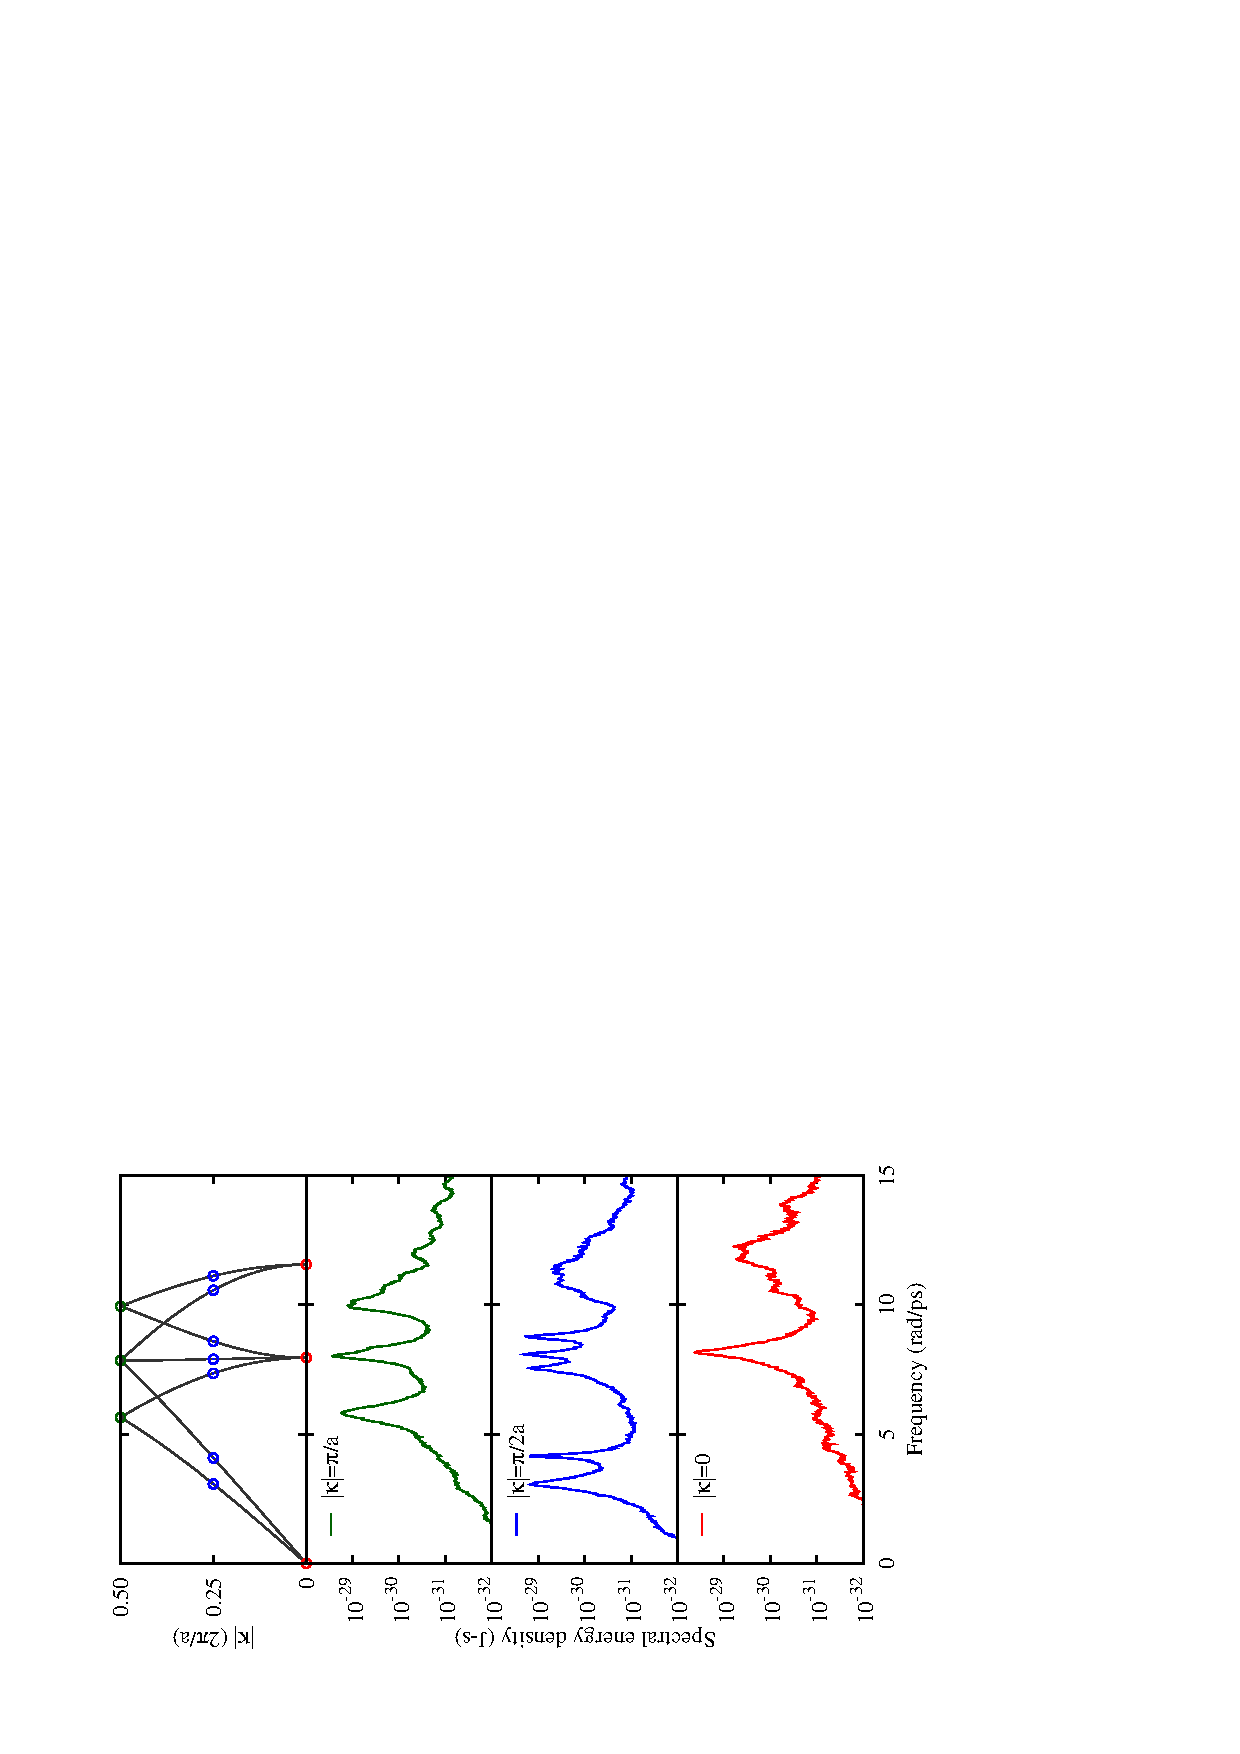
\includegraphics[angle=-90]{Ar_20K_4x4x4UC-SED}
\caption{\label{F:SED}DISPERSION CURVES ALONG THE [100] DIRECTION AND THE SPECTRAL
ENERGY DENSITY VERSUS FREQUENCY FOR WAVE VECTORS ALONG THE [100] DIRECTION
WITH MAGNITUDES OF $\pi/a$, $\pi/2a$, AND 0 FOR LENNARD-JONES ARGON AT A TEMPERATURE OF 20 K. THE MODES INDICATED WITH OPEN CIRCLES ON THE
DISPERSION CURVES CAN BE SEEN AS PEAKS IN THE SPECTRAL ENERGY DENSITY PLOTS.
THE ZERO FREQUENCY, ZERO WAVE VECTOR MODE CORRESPONDS TO BULK TRANSLATION AND DOES NOT EXIST IN MD SIMULATIONS WITH ZERO TOTAL MOMENTUM.
THE DATA IS SMOOTHED FOR VISUALIZATION BUT THE LORENTZIAN FUNCTIONS ARE FIT TO THE RAW DATA.}
\vspace*{-5mm}
\end{figure}

The results are plotted in Fig$.$ \ref{F:SED}. In the topmost sub-figure, the
dispersion curves, as predicted from quasi-harmonic LD, are shown. While
dispersion is normally plotted as frequency versus wave vector magnitude,
here we invert the axes for convenience. In the three remaining sub-figures
the SED is plotted versus frequency for wave vectors along the [100]
direction with magnitudes of $\pi/a$, $\pi/2a$, and 0.  The modes indicated
with open circles on the dispersion curves can be seen as peaks in the SED
plots.  The peaks below 10 rad/ps are well defined. The peaks at higher
frequencies are noisier.




%%%%%%%%%%%%%%%%%%%%% Final data %%%%%%%%%%%%%%%%%%%%%%%
\begin{table}[tb]
\caption{LENNARD-JONES ARGON PHONON PROPERTIES PREDICTED BY THE SPECTRAL
ENERGY DENSITY METHOD (SED), NORMAL-MODE DECOMPOSITION (NMD), AND ANHARMONIC
LATTICE DYNAMICS CALCULATIONS (ALD) AT A TEMPERATURE OF 20 K.}
\label{T:props}
\begin{center}
\begin{tabular}{|c|D{.}{.}{2} D{.}{.}{2}|D{.}{.}{2} D{.}{.}{2}|D{.}{.}{2} D{.}{.}{2}|}
  \hline
                   & \multicolumn{2}{c|}{SED} & \multicolumn{2}{c|}{MND} & \multicolumn{2}{c|}{ALD}\\ \hline
                   & \multicolumn{1}{c|}{$\omega_A$} & \multicolumn{1}{c|}{$\tau$} & \multicolumn{1}{c|}{$\omega_A$} & \multicolumn{1}{c|}{$\tau$} & \multicolumn{1}{c|}{$\omega_A$} & \multicolumn{1}{|c|}{$\tau$} \\
  \multicolumn{1}{|c|}{$|\pmb{\kappa}|$} & \multicolumn{1}{c|}{(1/ps)} & \multicolumn{1}{c|}{(ps)} & \multicolumn{1}{c|}{(1/ps)} & \multicolumn{1}{c|}{(ps)} & \multicolumn{1}{c|}{(1/ps)} & \multicolumn{1}{|c|}{(ps)} \\ \hline
  \multirow{2}{*}{0}                &  8.17 &  6.02 &  8.16 &  5.15 &  8.20 & 12.7  \\
                                    & 12.0  &  1.10 & 12.0  &  1.36 & 12.0  &  1.45 \\ \hline
  \multirow{7}{*}{$\frac{\pi}{a}$} &  3.07 &  5.45 &  3.06 &  7.43 &  3.11 &  6.74 \\
                                    &  4.15 & 13.9  &  4.15 &  8.85 &  4.24 & 15.3  \\
                                    &  7.55 &  6.43 &  7.55 &  5.20 &  7.59 & 10.3  \\
                                    &  8.09 &  8.09 &  8.08 &  5.43 &  8.12 & 14.0  \\
                                    &  8.77 &  8.82 &  8.77 &  4.62 &  8.81 & 16.5  \\
                                    & 10.8  &  3.21 & 10.8  &  1.93 & 10.9  &  2.60 \\
                                    & 11.4  &  1.19 & 11.4  &  1.29 & 11.4  &  1.57 \\ \hline
  \multirow{4}{*}{$\frac{\pi}{2a}$}  &  5.81 &  3.32 &  5.80 &  4.28 &  5.83 &  6.68 \\
                                    &  8.02 &  6.89 &  8.02 &  5.51 &  8.06 & 14.7  \\
                                    &  8.21 &  4.29 &  8.07 &  5.44 &  8.13 & 10.9  \\
                                    & 10.0  &  2.47 & 10.0  &  2.58 & 10.1  &  4.19 \\
  \hline
\end{tabular}
\end{center}
\end{table}

By fitting the peaks in the SED with Lorentzian functions using a least
squares method, we can extract the phonon frequencies and relaxation times
[see Eq$.$ \eqref{E:Lorentzian}].  The results are tabulated in Table
\ref{T:props} for all unique (i$.$e$.$, non-degenerate) modes.  The table
also includes predictions made using the normal-mode decomposition MD method
\cite{mcgaughey2004c} and anharmonic LD calculations \cite{turney2009a}. The
normal-mode decomposition predictions are made using the same simulations as
those used for the SED.  The agreement between the SED method and the
normal-mode decomposition method is generally good, as it should be since
these methods are similar.  In both methods, the system energy is being
mapped from direct space and time to reciprocal space and frequency.  The
agreement with the anharmonic LD predictions is not as good. This result may
be due to the low temperature approximations inherent in LD techniques
\cite{turney2009a}.  The normal-mode decomposition method also loses accuracy
at higher temperatures because the quasi-harmonic phonon frequencies and
polarization vectors are used to perform the energy mapping
\cite{turney2009a}.  The SED method, however, does not suffer from this
limitation and should be applicable at higher temperatures as long as the
weakly-interacting phonon interpretation is valid.

\section*{SUMMARY}

In this paper, we derived the spectral energy density and the relationship
between the spectral energy density and the phonon frequencies and relaxation
times. We then calculated the spectral energy density for Lennard-Jones argon
at a temperature of 20 K and used it to obtain the phonon frequencies and
relaxation times, as shown in Fig$.$ \ref{F:SED} and Table \ref{T:props}. The
frequencies are in excellent agreement with those predicted using other
techniques, while the relaxation times show reasonable agreement. Further
work is required to understand the differences.

The advantages of the SED method are that (i) other than the the wave
vectors, which can be determined from the system geometry, no phonon
properties need to be known {\em a priori} and (ii) it naturally incorporates
the full effect of anharmonicity (through the MD simulation). The main
disadvantage is that the different dispersion branches are not handled
separately. Instead, the SED at each wave vector contains information for all
dispersion branches. As a result, it can be difficult to identify or fit
Lorentzian functions to closely-spaced peaks in the SED. Though not
essential, knowledge of the quasi-harmonic frequencies can help to identify
the unique peaks in the SED as well as the degeneracy.

%%%%%%%%%%%%%%%%%%%%%%%%%%%%%%%%%%%%%%%%%%%%%%%%%%%%%%%%%
\begin{acknowledgment}
This work is supported by the Pennsylvania Infrastructure Technology
Alliance, a partnership of Carnegie Mellon, Lehigh University, and the
Commonwealth of Pennsylvania's Department of Community and Economic
Development (DCED),  Advanced Micro Devices (AMD), and the National Science
Foundation through a graduate fellowship to JAT.
\end{acknowledgment}

%%%%%%%%%%%%%%%%%%%%%%%%%%%%%%%%%%%%%%%%%%%%%%%%%%%%%%%%%
\bibliographystyle{asmems4}

\bibliography{jan10}

%%%%%%%%%%%%%%%%%%%%%%%%%%%%%%%%%%%%%%%%%%%%%%%%%%%%%%%%%

\end{document}
